\documentclass[polish,envcountsect,10pt]{beamer}
    \usepackage[T1]{fontenc}
    \usepackage{polski}
    \usepackage{babel}
    \usepackage{tikz}
    \usetheme{Warsaw}
    \title{Problem chińskiego listonosza (PCL)}
    \author{184657 Wojciech Panfil}
    \date{Gdańsk, 9.11.2023}
\begin{document}

\frame{\titlepage}

\begin{frame}{Graf}
    Graf - matematyczna struktura danych składająca się z wierzchołków oraz krawędzi.
    \begin{itemize}
        \item Wierzchołki (węzły) reprezentowane są jako punkty i należą do zbioru $V$.
        \item Krawędzie (łuki) łączą wierzchołki i należą do zbioru $E$.
    \end{itemize}
    \begin{center}
        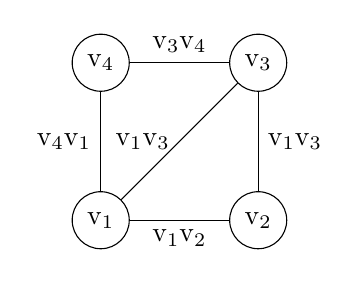
\begin{tikzpicture}
            \node[draw, circle] (v1) at (0,0) {v\textsubscript{1}};
            \node[draw, circle] (v2) at (2,0) {v$_2$};
            \node[draw, circle] (v3) at (2,2) {v$_3$};
            \node[draw, circle] (v4) at (0,2) {v$_4$};

            \draw (v1) -- (v2) node[midway, below] {v$_1$v$_2$};
            \draw (v2) -- (v3) node[midway, right] {v$_1$v$_3$};
            \draw (v3) -- (v4) node[midway, above] {v$_3$v$_4$};
            \draw (v4) -- (v1) node[midway, left] {v$_4$v$_1$};
            \draw (v1) -- (v3) node[midway, left] {v$_1$v$_3$};
        \end{tikzpicture}
    \end{center}
    \begin{itemize}
        \item G = ($V$ , $E$)
        \item $V$ = \{v$_1$, v$_2$, v$_3$, v$_4$\}
        \item $E$ = \{v$_1$v$_2$, v$_1$v$_3$, v$_3$v$_4$, v$_4$v$_1$, v$_1$v$_3$\}
    \end{itemize}
\end{frame}

\begin{frame}{Graf skierowany (digraf)}
    \begin{itemize}
    \item Graf skierowany, nazywany również digrafem, to rodzaj grafu, w którym krawędzie mają określony kierunek.
    \item W digrafie każda krawędź ma źródło (początkowy wierzchołek) i cel (końcowy wierzchołek).
    \item Krawędzie w digrafie są reprezentowane jako strzałki, które wskazują kierunek od źródła do celu.
    \item Digrafy są używane do modelowania relacji, w których kierunek ma znaczenie, na przykład w sieciach telekomunikacyjnych czy ścieżkach przesyłu danych.
    \end{itemize}

    \begin{center}
        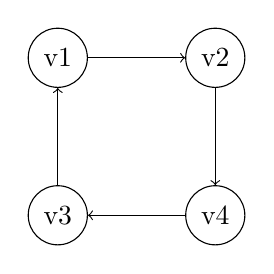
\begin{tikzpicture}
            \node[draw, circle] (v1) at (0,2) {v1};
            \node[draw, circle] (v2) at (2,2) {v2};
            \node[draw, circle] (v3) at (0,0) {v3};
            \node[draw, circle] (v4) at (2,0) {v4};

            \draw[->] (v1) -- (v2);
            \draw[->] (v2) -- (v4);
            \draw[->] (v4) -- (v3);
            \draw[->] (v3) -- (v1);
        \end{tikzpicture}
    \end{center}
\end{frame}

\begin{frame}{Graf ważony}
    \begin{itemize}
        \item Graf ważony to rodzaj grafu, w którym każda krawędź ma przypisaną wagę lub koszt.
        \item Wagi krawędzi mogą reprezentować różne parametry, takie jak odległość, koszt, czas, lub dowolną inną miarę.
        \item Wagi krawędzi są często reprezentowane na krawędziach lub przy użyciu etykiet.
        \item Grafy ważone używane są w różnych dziedzinach, takich jak planowanie tras, sieci komunikacyjne, i analiza danych.
    \end{itemize}
    \begin{center}
        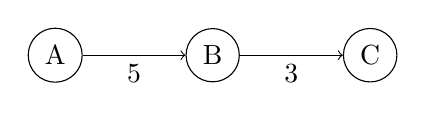
\begin{tikzpicture}
            \node[draw, circle] (A) at (0,0) {A};
            \node[draw, circle] (B) at (2,0) {B};
            \node[draw, circle] (C) at (4,0) {C};

            \draw[->] (A) -- (B) node[midway, below] {5};
            \draw[->] (B) -- (C) node[midway, below] {3};
        \end{tikzpicture}
    \end{center}
\end{frame}

\begin{frame}{Graf spójny}
    \begin{itemize}
        \item Graf spójny (lub graf spójny) to graf, w którym istnieje ścieżka między każdą parą wierzchołków.
        \item Oznacza to, że w grafie spójnym można przejść od dowolnego wierzchołka do dowolnego innego wierzchołka, przechodząc po krawędziach.
        \item Grafy spójne są jednym spójnym "kawałkiem" bez izolowanych wierzchołków lub podgrafów, które nie są ze sobą połączone.
    \end{itemize}
    \begin{center}
        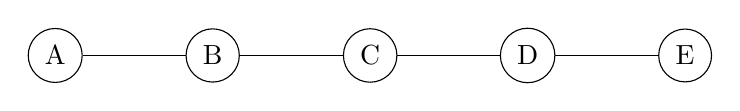
\begin{tikzpicture}
            \node[draw, circle] (A) at (0,0) {A};
            \node[draw, circle] (B) at (2,0) {B};
            \node[draw, circle] (C) at (4,0) {C};
            \node[draw, circle] (D) at (6,0) {D};
            \node[draw, circle] (E) at (8,0) {E};
        
            \draw (A) -- (B);
            \draw (B) -- (C);
            \draw (C) -- (D);
            \draw (D) -- (E);
        \end{tikzpicture}

        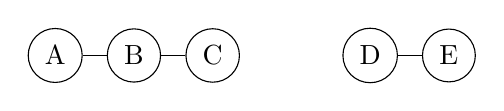
\begin{tikzpicture}
            \node[draw, circle] (A) at (0,0) {A};
            \node[draw, circle] (B) at (1,0) {B};
            \node[draw, circle] (C) at (2,0) {C};
            \draw (A) -- (B);
            \draw (B) -- (C);

            \node[draw, circle] (D) at (4,0) {D};
            \node[draw, circle] (E) at (5,0) {E};
            \draw (D) -- (E);
          \end{tikzpicture}
    \end{center}
\end{frame}

\end{document}